\chapter{Results}
\section{\label{section:Results from Simulation}Results from Simulation}
%\subsection{\label{Pheromone Only Parameters}Pheromone Only Parameters}
We configured the simulation settings as close as we can with the experimental setup of \textit{P. rugosus}, \textit{P. maricopa} and \textit{P. desertorum}. Then we have compared the result of change point analysis on \textit{foraging rate}, \textit{change in foraging rate}, \textit{constant detrended foraging rate }, \textit{constant detrended change in foraging rate}, \textit{linear detrended foraging rate} and \textit{linear detrended change in foraging rate}.\par
\begin{figure}[]
	\includegraphics[width=\textwidth,height=0.5\textheight]{PheromoneOnly/AllPlot.png}
	\caption{Comparison of change point detection method for pheromone only parameters. Outliers are skipped to provide a better indication of differences. The time in seconds represents the difference between a pheromone laying event followed by a detection of change point in the foraging rate.}
\end{figure} 
Figure $4.1$ compares the results of four different methods on a pheromone only simulated environment for \textit{P. rugosus}. We can see that, \textit{constant detrending} detects change points which is closer to the pheromone laying event. The result of \textit{constant detrending with change in foraging rate} is closer to the \textit{constant detrending}, but \textit{linear detrending} and \textit{linear detrending with change in rate} doesn't perform well in this environmental settings.\par 

The average difference of pheromone laying event followed by a change point detection for \textit{constant detrending} method is $47.5$, $60$ and $81.5$ for one pile, four large piles and sixteen piles. It is also observed that, the range of time difference between a pheromone laying event followed by a change point detection event is also significantly reduced.\par 
We observe similar phenomenon for \textit{P. maricopa} and \textit{P. desertorum}. The box plots of comparison for these two species are provided in the appendices. The outliers are removed from the figure to make the figure more informative. The detailed figure with the outliers are provided in the appendices.\par 
We compare the result with the change point detection in raw foraging rate. We observe that, the average time difference between change point detection and pheromone laying event is similar to \textit{constant detrending}. \par
\begin{figure}[]
	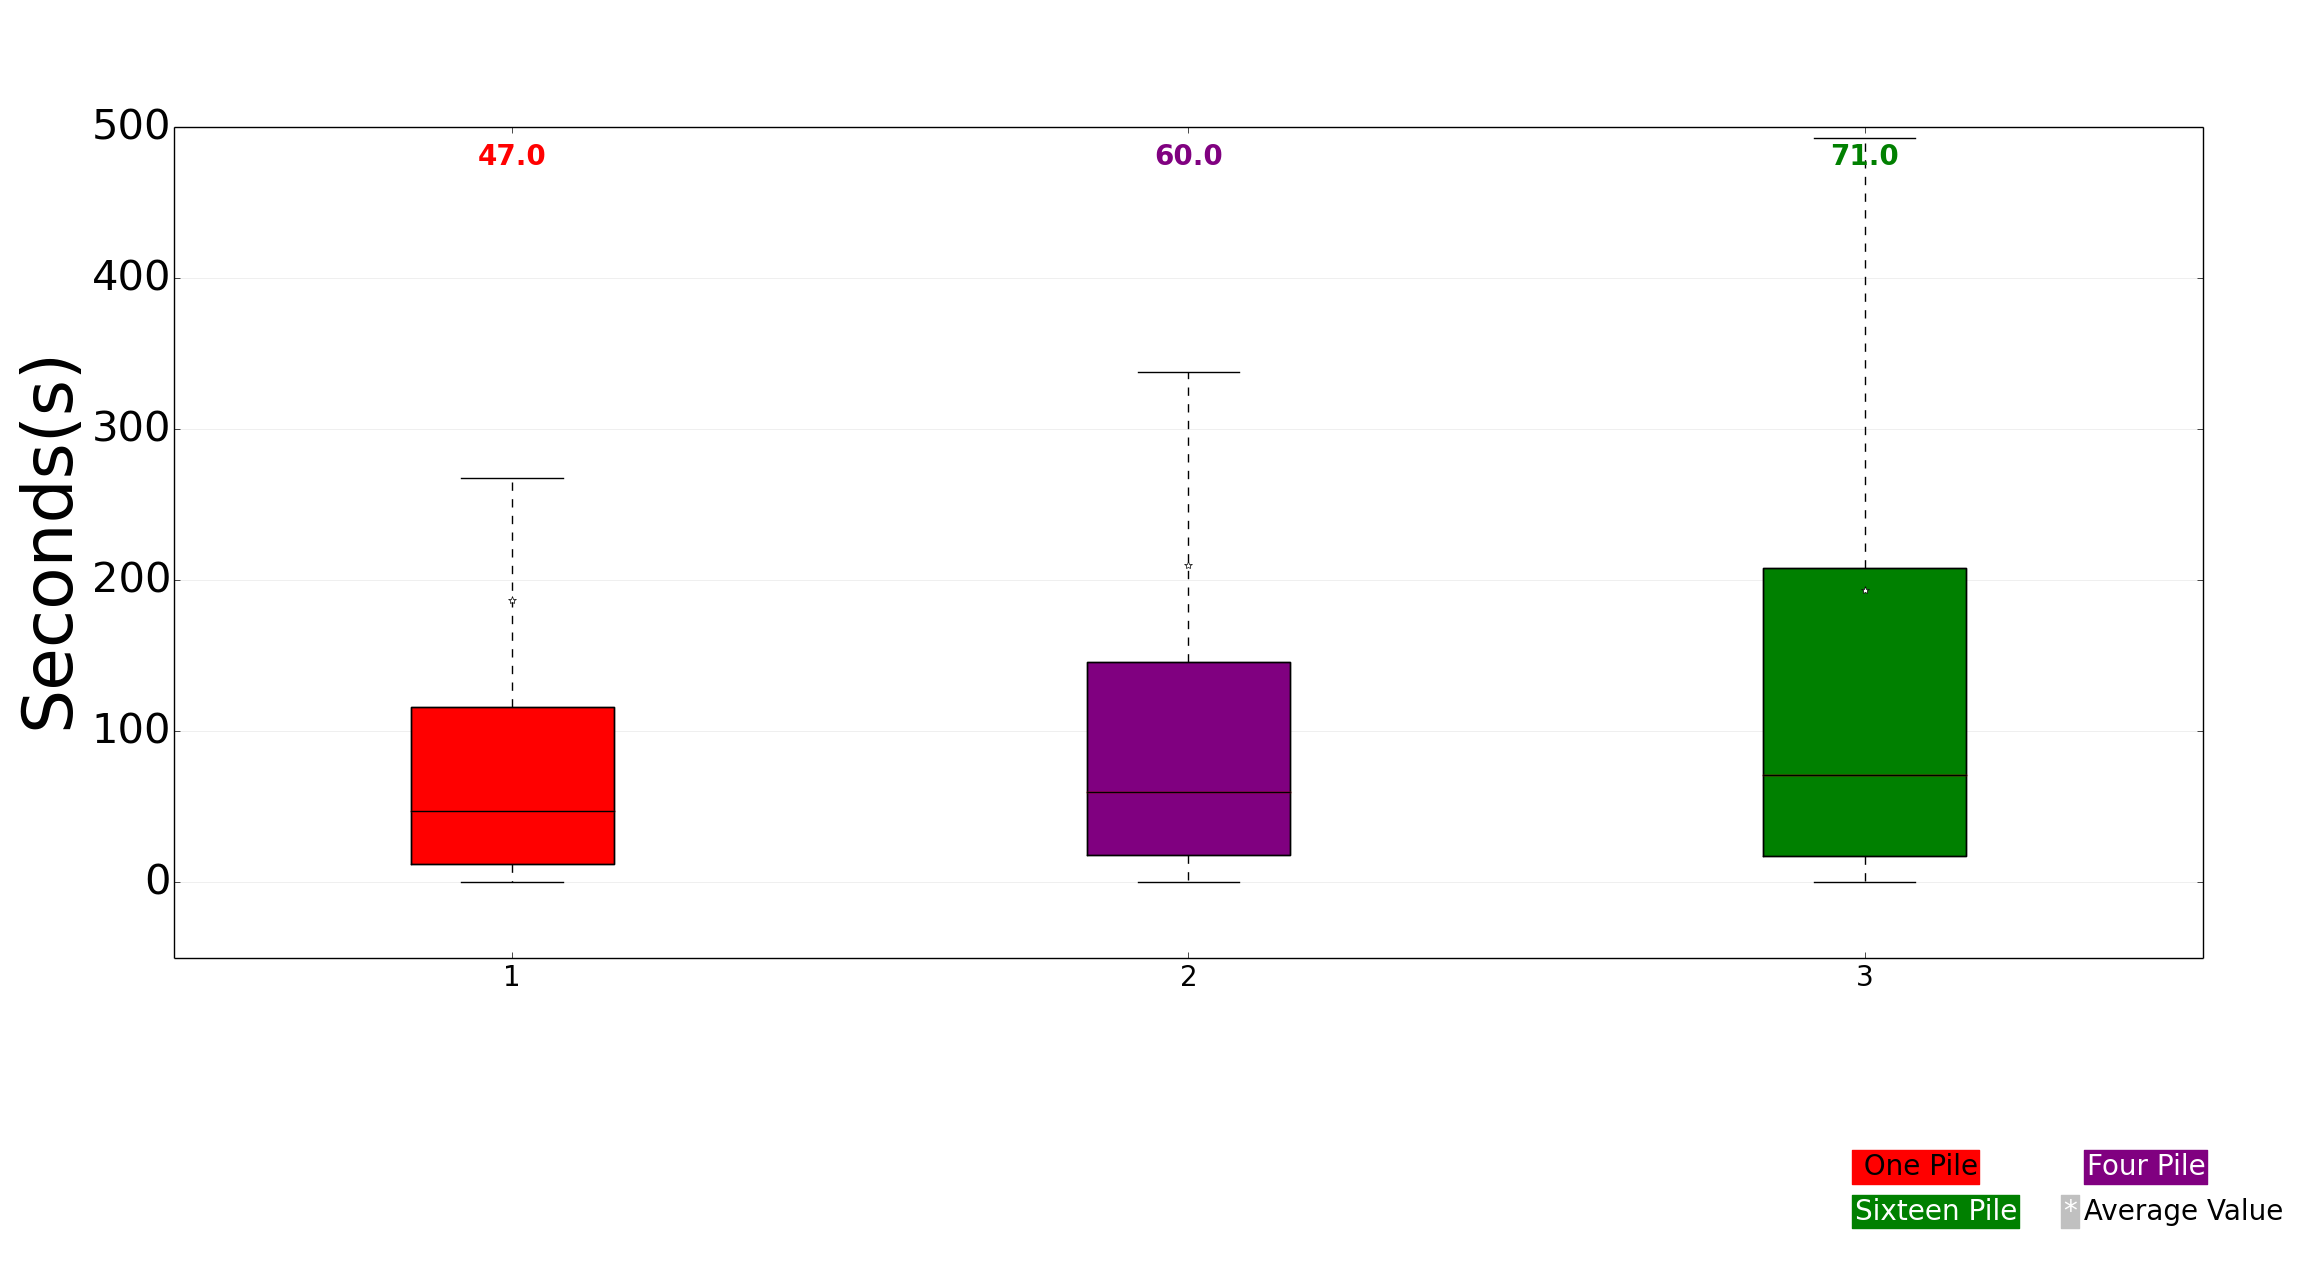
\includegraphics[width=\textwidth,height=0.5\textheight]{PheromoneOnly/RawFit/12Ant_PhOnly_CP.png}
	\caption{Enlarged view of efficiency of change point detection algorithm on raw foraging rate. The time in seconds represents the difference between a pheromone laying event followed by a detection of change point in the foraging rate.}
\end{figure}
We have also evaluated four different methods based on the four categories mentioned in section $3.7$.
As we can see from figure $4.3$ in \textit{constant detrending} , $15\%$ of the time change points are detected within 10 seconds of laying pheromone, whereas, in \textit{linear detrending} , it is only $9\%$. \textit{Constant detrending}  also has significant improvement over \textit{linear detrending}  in \textit{Catagory $11-300$}. $74\%$ of the time, changes points are detected with eleven to three hundred seconds of laying pheromone while using \textit{constant detrending} , on the other hand, using \textit{linear detrending} it is only $50\%$. In \textit{catagory $>300$} the error is $6\%$ for \textit{constant detrending} , whereas, it is $21\%$ for \textit{linear detrending}. \par
\begin{figure}[h]
	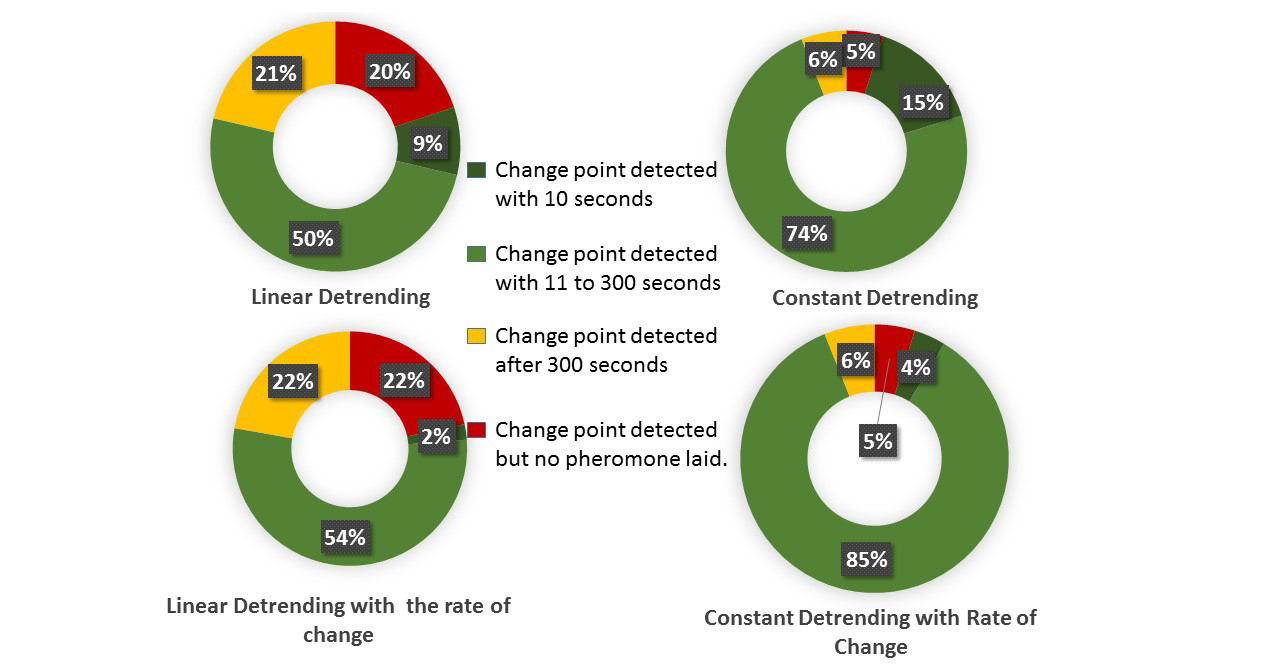
\includegraphics[height=0.35\textheight]{DonutCharts/Slide2.JPG}
	\caption{Efficiency chart for change point detection methods on a large pile of 256 seeds. This result is generated from the simulated data of pheromone only parameters, configured for \textit{P. rugosus}}
\end{figure}
\begin{figure}[H]
	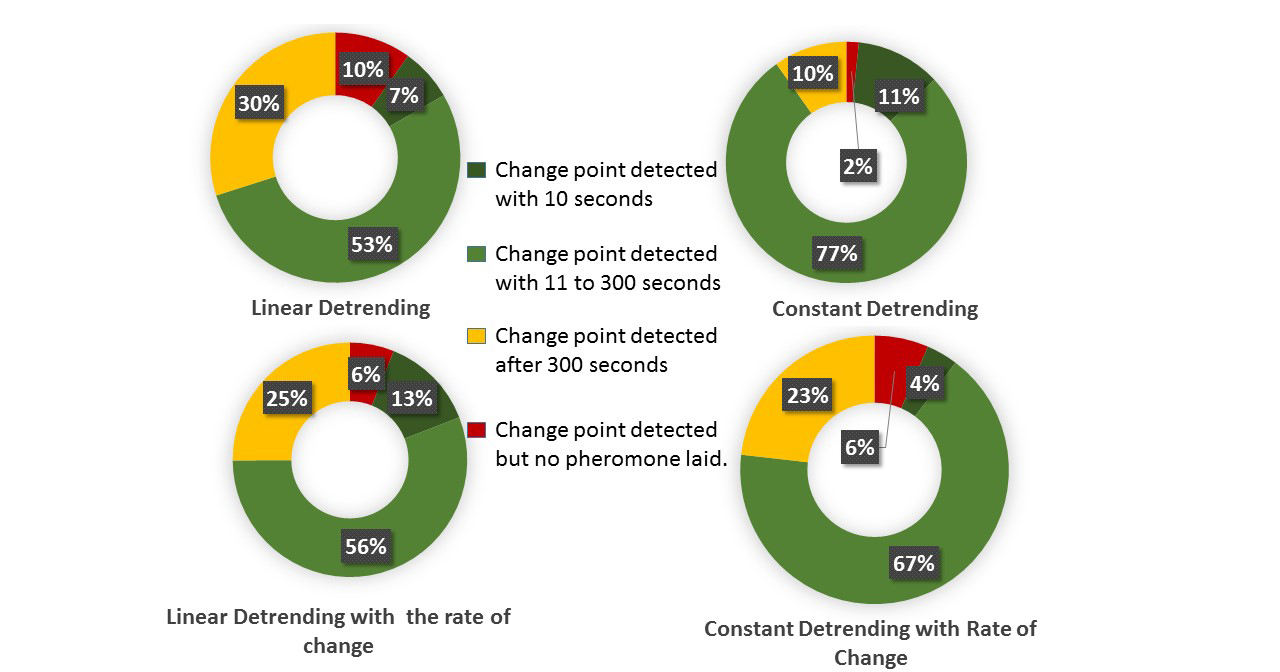
\includegraphics[width=\linewidth, height=0.4\textheight]{DonutCharts/Slide3.JPG}
	\caption{Efficiency chart for change point detection methods on four medium  piles of 64 seeds. This result is generated from the simulated data of pheromone only parameters, configured for \textit{P. rugosus}}
\end{figure}
Performance of \textit{constant detrending method} and \textit{constant detrending method with difference in rate} is similar, if we consider \textit{categories $\le 10$} and \textit{catagory $11-300$}. But \textit{constant detrending} does significantly better than \textit{constant detrending with change of foraging rate} in detecting change points for four piles and sixteen piles in the simulated environment.\par
\begin{figure}[H]
	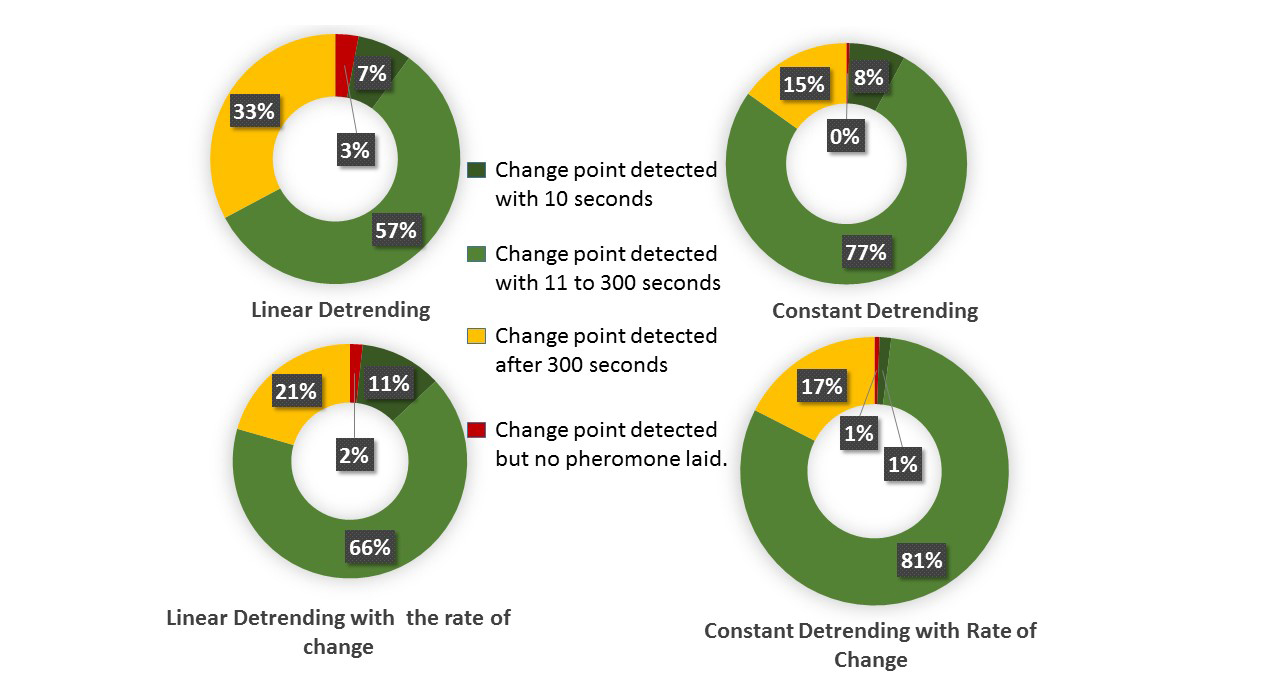
\includegraphics[width=\linewidth, height=0.4\textheight]{DonutCharts/Slide4.JPG}
	\caption{Efficiency chart for change point detection methods on sixteen small piles of 16 seeds. This result is generated from the simulated data of pheromone only parameters, configured for \textit{P. rugosus}}
\end{figure}
From figure $4.4$ and figure $4.5$ we can observe that, the performance of \textit{constant detrending} combined in \textit{category $\le 10$} and \textit{catagory $11-300$} is better than performance of \textit{constant detrending with change in foraging rate} combined in these two categories. Also from figure $4.4$ and $4.5$ we can see that \textit{constant detrending} does better in \textit{category $>300$} than \textit{constant detrending with change in foraging rate}. \par
If we look at the performance of the four methods over these categories in phermone only simulated environments, for \textit{P. maricopa} and \textit{P. desertorum} we observe similar pattern of performances. The results for \textit{P. maricopa} and \textit{P. desertorum} are provided in the appendices.\par  
\begin{figure}[]
	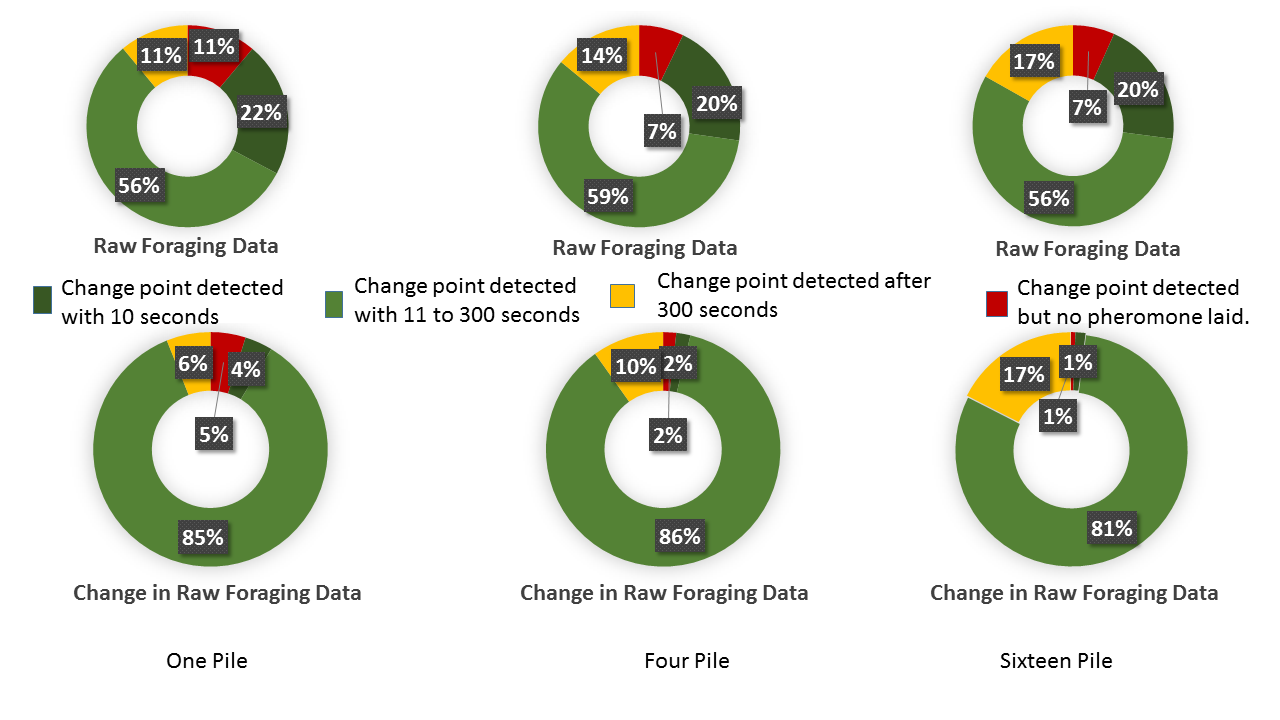
\includegraphics[width=\linewidth, height=0.4\textheight]{PheromoneOnly/RawFit/12AntsRawFitPHOnly.PNG}
	\caption{Efficiency chart for change point detection methods on foraging rate and change in foraging rate. This result is generated from the simulated data of pheromone only parameters, configured for \textit{P. rugosus}}
\end{figure}
Figure $4.6$ shows efficiency of change point detection algorithm on \textit{raw foraging rate} and \textit{change in foraging rate} in pheromone only experiments. We observe that, the performance is better for \textit{change in foraging rate}. \par
Figure $4.7$ shows the comparison of four different methods on a simulated environment with both memory and communication for \textit{P. rugosus}. From this figure it is clearly visible that \textit{constant detrending} does better in detecting the change points than any other methods. As a matter of fact, \textit{constant detrending} does better in memory plus communication environment than the communication only environment.\par 

\begin{figure}[H]
	\includegraphics[width=\textwidth,height=0.6\textheight]{AllParameters/AllPlot.png}
	\caption{Comparison of change point detection methods without outliers for \textit{pheromone plus sitefidelity} parameters . The time in seconds represents the difference between a pheromone laying event followed by a detection of change point in the foraging rate.}
\end{figure}
\begin{figure}
	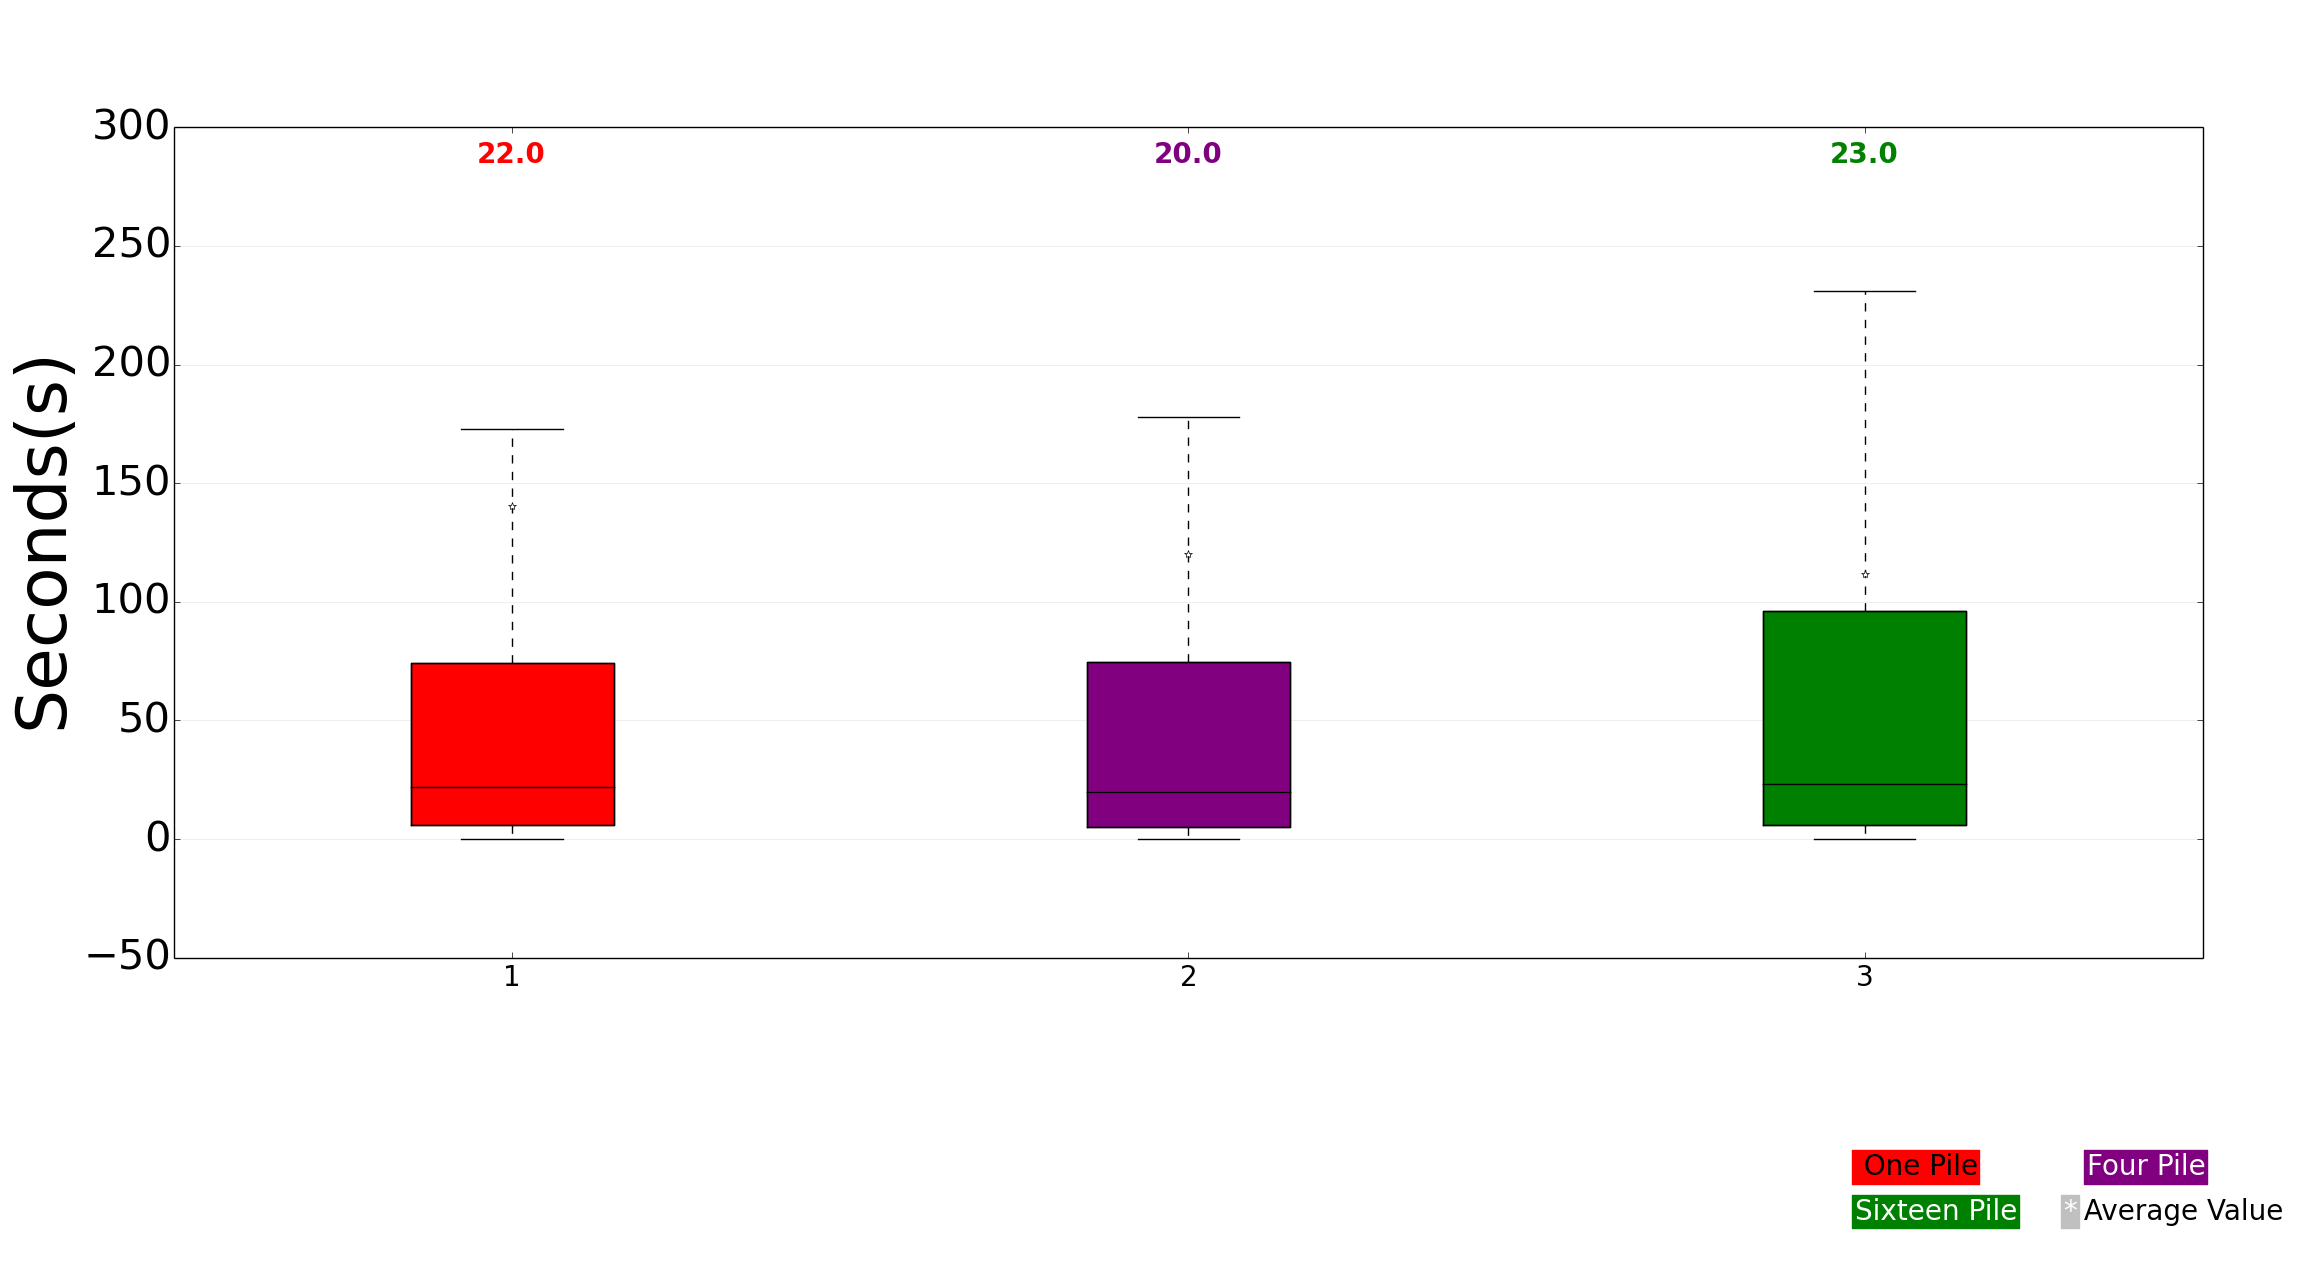
\includegraphics[width=\textwidth,height=0.4\textheight]{AllParameters/RawFit/12Ants_SFandPH_WithRate_RoundTripWindow.png}
	\caption{Enlarged view of efficiency of change point detection algorithm on \textit{raw foraging rate} on simulation data of 12 ants. The time in seconds represents the difference between a pheromone laying event followed by a detection of change point in the foraging rate. Compared to figure 4.7 change point detection on raw data detects changes fastest.}
\end{figure}
\begin{figure}[h]
		\centering
		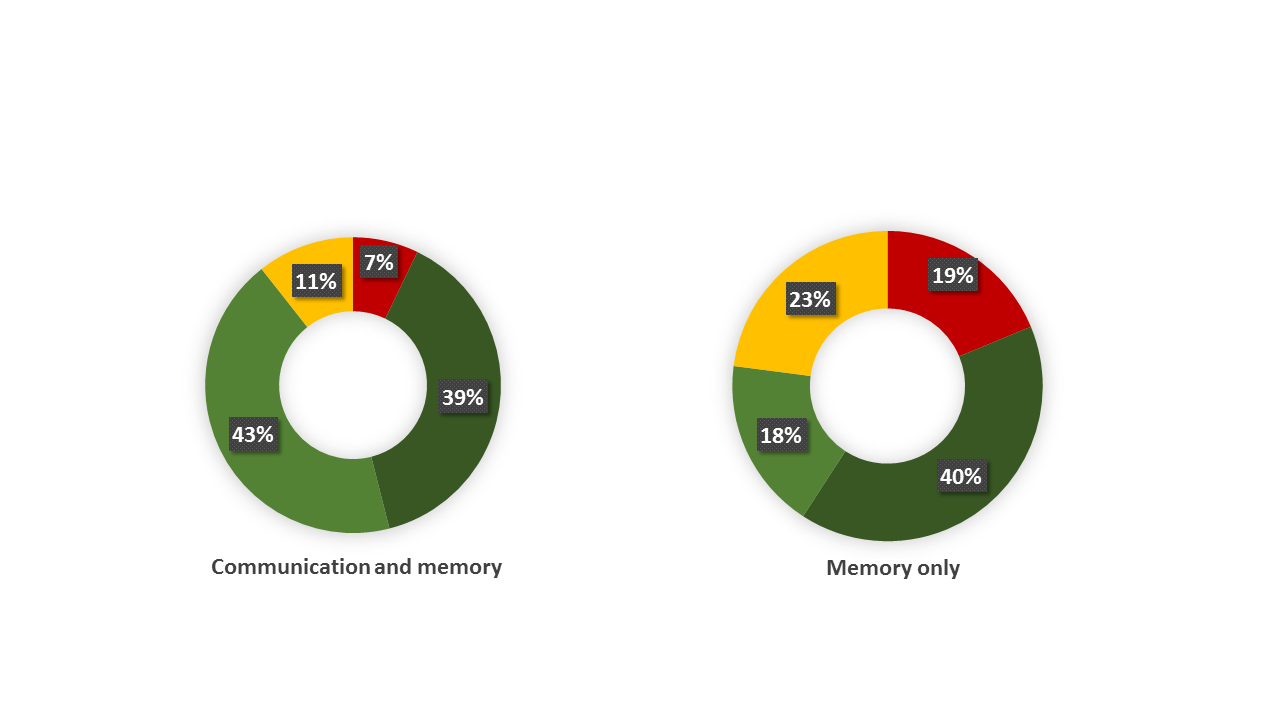
\includegraphics[width=\linewidth]{Comparison.PNG}
	\caption{Figure on the left is the efficiency chart of the change point detection algorithm on \textit{raw foraging rate with no detrending} for one large pile of 256 seeds. The data is generated from the simulation of pheromone plus site fidelity parameters of \textit{P. rugosus}. 
		Figure on the right is the efficiency chart of change point detection algorithm on \textit{raw foraging rate with no detrending} for one large pile of 256 seeds. The figure is generated by analyzing the simulated data of sitefidelity only parameters for \textit{P. rugosus}. }
	\label{fig:fig}
\end{figure}
\begin{figure}
	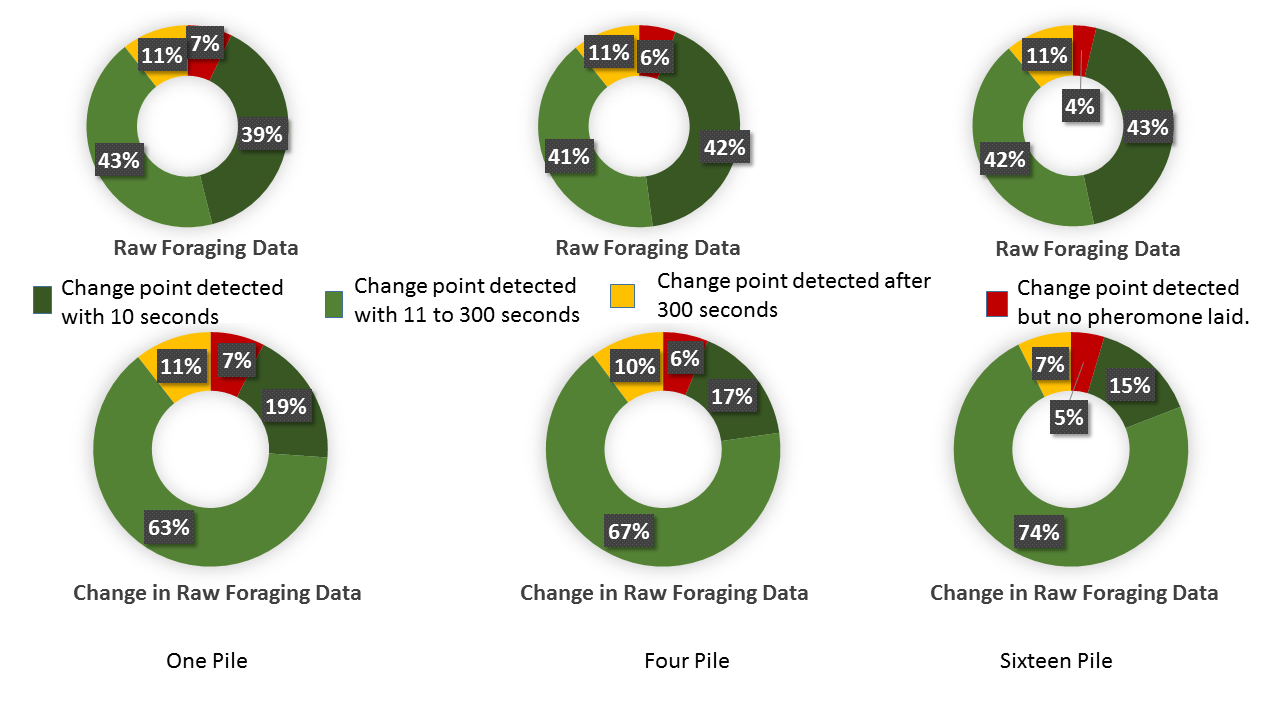
\includegraphics[width=\textwidth,height=0.4\textheight]{AllParameters/RawFit/12AntsRawFitSFAndPH.PNG}
	\caption{Efficiency of change point detection algorithm for detecting pheromone using\textit{ raw foraging rate} and \textit{change in raw foraging rate}, in memory and communication parameters.}
\end{figure}
\begin{figure}
	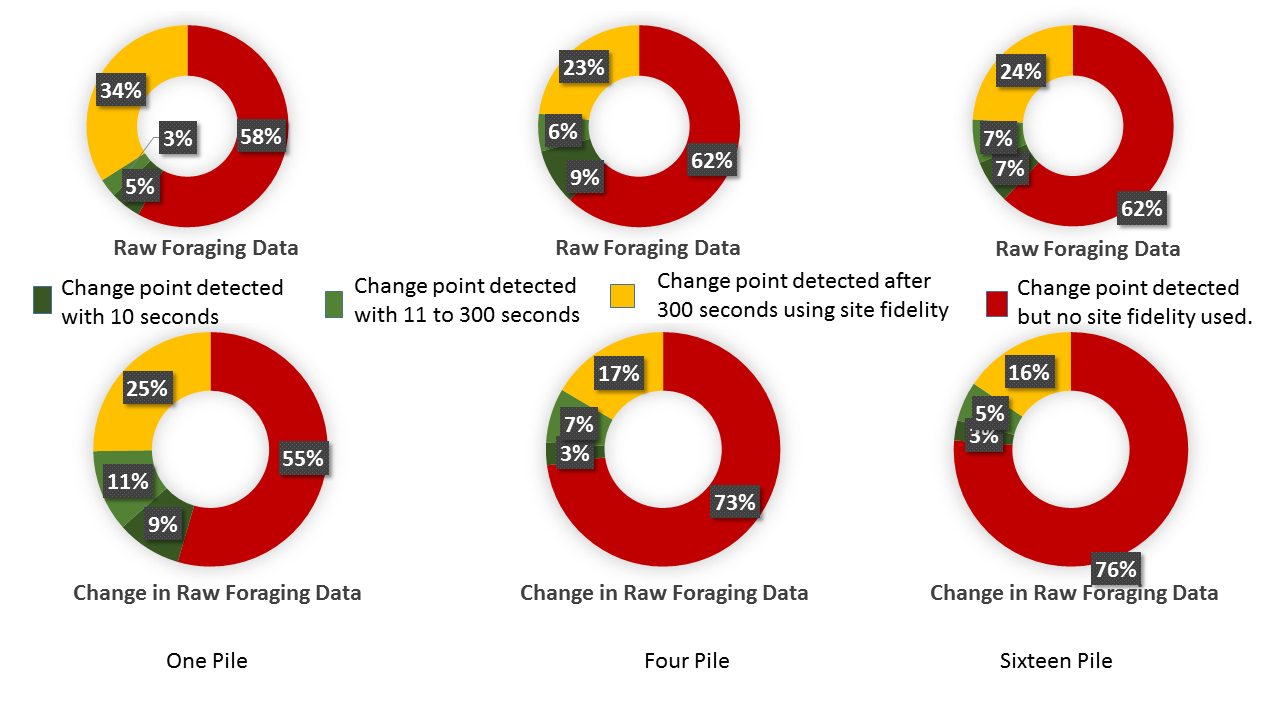
\includegraphics[width=\textwidth,height=0.4\textheight]{AllParameters/RawFit/SiteFidelityGraph.PNG}
	\caption{Efficiency of change point detection algorithm on raw data for detecting site fidelity in memory and communication parameters.}
\end{figure}
\begin{figure}[h]
	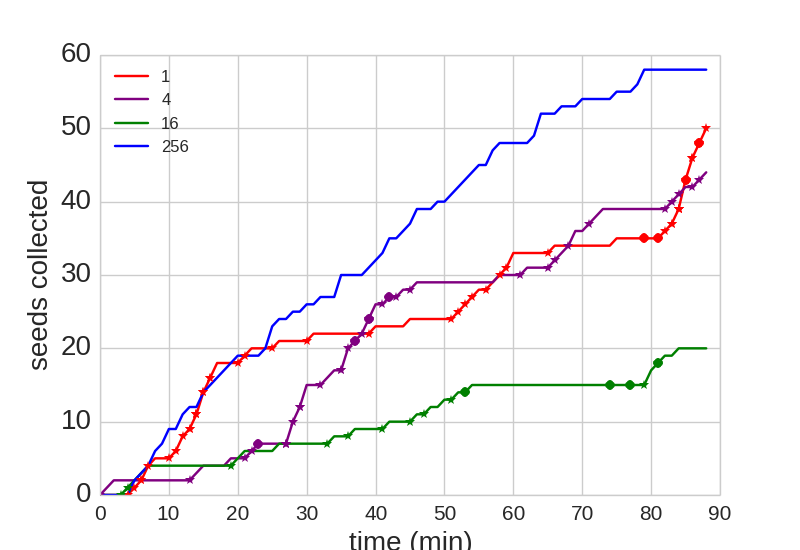
\includegraphics[height=0.4\textheight,width=\linewidth]{NewResult/RandomSeed_43109511.png}
	\caption{A plot of seed collection from simulation of 12 simulated ants. The stars in the foraging data represent the pheromone laying event and circles represent detection of change points using the binary segmented cumulative sum method on raw data.}
\end{figure}
We have analyzed the efficiencies of all four methods for communication plus memory environmental settings. We observe that \textit{constant detrending} and \textit{constant detrending with change in foraging rate} does significantly better than the other two methods. But in \textit{category $>300$} and catagory None, \textit{constant detrending} does better than \textit{constant detrending with change in rate}. We observe that the error is 0\% for \textit{constant detrending}, whereas it is 1\% for \textit{constant detrending with change in foraging rate}. \textit{Constant detrending} also surpasses \textit{constant detrending with change in foraging rate} in the combined result of \textit{category $\le 10$} and \textit{category $11-300$}. We observe, the similar pattern of performances for four piles and sixteen piles. \par
Figure $4.8$ shows the efficiency of change point detection algorithm on foraging rate. We observe, time to detect the change points is better than \textit{constant detrending}. \par%upto this
Figure \textit{4.9(a)} is the efficiency chart for \textit{foraging rate with no detrending} for one large pile on pheromone plus site fidelity environment. The result of other piles for \textit{P. rugosus} have similar pattern. We have mentioned those in appendices. In figure \textit{4.9(b)} we demonstrate our model\textquotesingle s efficiency in detecting the change points when only site fidelity is used for \textit{P. rugosus} on one large pile of 256 seeds.\par 
In memory only environment when no pheromone is used, agents use memory extensively. For this reason, when they start collecting seeds, their foraging rate goes up because of the extensive use of internal memory. Which is why \textit{constant detrending} also method detects change points in site fidelity only environment. So we have also measured the efficiency of all methods by measuring the difference between a use of site fidelity and followed by a change point. From figure 4.9(b), we have observed that 58\% of the time a change point is detected after the first use of site-fidelity.\par  
The performance rating is similar for \textit{P. maricopa} and \textit{P. desertorum}. Results for these two species are provided in the appendices. \par
To validate which method is better in detecting only pheromone but no site-fidelity event, we have also calculated the time difference between site fidelity and followed by a change point detection event for memory plus communication environment. From figure $4.10$ we observe that, only for few experiments it detects change points for the use of memory. This data is generated by applying the change point detection algorithm on \textit{foraging rate} and \textit{change in foraging rate}. We observe similar pattern for \textit{constant detrending} method. Although we miss some of the change points when we use the \textit{foraging rate with no detrending} or \textit{change in foraging rate with no detrending}, it is better because we do not detect much of the site fidelity events in this method.\par 
We have varied the number of ants to observe the change in the foraging rate in the simulation. We have performed the simulation with 96 ants and 48 ants. We have observed that in the simulation with 96 ants, they collect more random seeds than the seeds that are clumped. A reason for this is when the number of ants is too large, the rate of collision increases between them while they try to forage from a clumped food source. The performance is little better when we ran the experiment with 48 ants. They tend to collect seeds from the clumped food distribution. \par

We have applied the change point detection algorithm on the foraging rate of these two types of simulations, keeping the parameters for change point detection algorithm same. We observe that the average time difference between a pheromone laying event followed by a change point detection algorithm increases for 48 ants. And it is increased more for 96 ants. \par

We ran the simulation for 96 and 48 ants with site fidelity only parameters, we observe that they don't use the site fidelity often to recruit. Even though they use, it does not effect in their foraging rate. Although we have detected a few change points in their foraging rate, the accuracy of the algorithm is very low in the simulation for size fidelity only parameters. The results are included in the appendices. \par
The change point detection algorithm on raw foraging data detects the pheromone laying event fastest in pheromone only experiments. It also detects pheromone in memory and communication only environment. However, It rarely detects change points for sitefidelity in memory and sitefidelity experiments. It also detects change points in memory only experiments because sitefideity is used so often in these experiments. \par
Because it is the best at detecting changepoints, we use the binary segmented cumsum change point detection algorithm on raw data to detect recruitment in the field data. 
 
\section{\label{section:Results from Field Data}Results from Field Data} 
We applied the change point detection algorithm on the change of foraging rate in field data. The parameters are kept same as simulations for the change point detection method. We are able to detect change points in 10 experiments out of 11 for \textit{P. desertorum}. For \textit{P. maricopa}, we detected change points in 10 experiments out of 11 and for \textit{P. rugosus} we are able to detect change points in 11 experiments out of 13. Table $4.2$ shows the detail of the results for field data.\par
\begin{table}[H]
	\footnotesize
	\begin{tabular}{|c|c|c|c|}
		\hline
		\multicolumn{4}{|c|}{\textit{P. desertorum}} \\ \hline
		Experiment & One & Four & Sixteen \\ \hline
		DP15\_070709 & 4 & 2 & 2 \\ \hline
		DP10\_0606 & 3 & 3 & 2 \\ \hline
		DP14\_0606 & 2 & 2 & 2 \\ \hline
		DP15\_0604 & 2 & 0 & 2  \\ \hline   
		DP15\_0617 & 1 & 2 & 2 \\ \hline
		DPC\_070109 & 2 & 1 & 2  \\ \hline
		DP15\_070809 & 3 & 2 & 2  \\ \hline
		DP16\_0610 & 2 & 2 & 2  \\ \hline
		DPB\_070809 & 2 & 2 & 2  \\ \hline
		DP9\_0603 & 0 & 3 & 2  \\ \hline
	\end{tabular}
	\hfill
	\begin{tabular}{|c|c|c|c|}
		\hline
		\multicolumn{4}{|c|}{\textit{P. maricopa}} \\ \hline
		Experiment & One & Four & Sixteen \\ \hline
		MP8\_0609 & 3 & 3 & 4 \\ \hline
		MP9\_0528 & 2 & 2 & 1 \\ \hline
		MP9\_0602 & 1 & 2 & 2 \\ \hline
		MP9\_0611 & 2 & 2 & 1  \\ \hline   
		MP9\_0620 & 2 & 2 & 2 \\ \hline
		MPE\_24Jul09 & 2 & 2 & 2  \\ \hline
		MP4\_0527 & 2 & 2 & 2  \\ \hline
		MP7\_0620 & 1 & 2 & 2  \\ \hline
		MP8\_0527 & 1 & 1 & 1  \\ \hline      
		MPX\_0624 & 2 & 2 & 3  \\ \hline  
	\end{tabular}
	\hfill
	\\ \\
	\begin{center}
		\begin{tabular}{|c|c|c|c|}
			\hline
			\multicolumn{4}{|c|}{\textit{P. rugosus}} \\ \hline
			Experiment & One & Four & Sixteen \\ \hline
			RP6\_0609 & 2 & 2 & 2 \\ \hline
			RP7\_0610 & 3 & 2 & 1 \\ \hline
			RP10\_0527 & 2 & 2 & 2 \\ \hline
			RP10\_0528 & 1 & 2 & 2  \\ \hline   
			RP10\_0604 & 2 & 0 & 1 \\ \hline
			RP12\_0602 & 2 & 2 & 2  \\ \hline
			RP14\_0610 & 2 & 1 & 2  \\ \hline  
			RP16\_0612 & 2 & 2 & 2  \\ \hline
			RP19\_0618 & 3 & 2 & 2  \\ \hline
			RS23\_0821 & 2 & 2 & 2  \\ \hline 
			RP17\_0617 & 1 & 3 & 2  \\ \hline 
		\end{tabular}
	\end{center}
	\caption{This table represents the number of change points detected in each of the field experiment of \textit{P. desertorum}, \textit{P. maricopa} and \textit{P. rugosus}. For \textit{P. desertorum}, we are able to detect change points in 10 experiments out of 11. For \textit{P. maricopa} it is 10 out of 11. For \textit{P. rugosus} it is 11 out of 13. The numbers conclude how many times change points are detected for a pile type in each experiment.}
\end{table}
\begin{figure}[h]
 	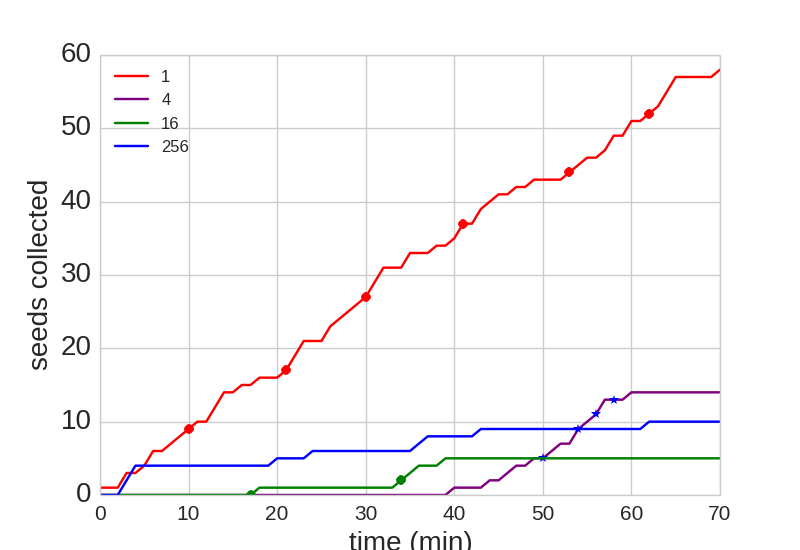
\includegraphics[height=0.4\textheight,width=\linewidth]{NewResult/DP9.png}
 	\caption{A plot of seed collection from one of the field experiment of \textit{P. desertorum} with change points indicate with circles.}
\end{figure}
 
We ran 500 simulated experiment to generate the data for each species. And we are able to detect change points in all of the experiments. In the field experiments we were also able to detect change points for most of the experiments. 
This suggests all three species are either using pheromones for all pile sizes or they exclusively use sitefidelity, but use it in large amounts that generate change points.
